\section{Referencia de la Clase Pagos\-List}
\label{classPagosList}\index{PagosList@{PagosList}}
Muestra y administra el listado de pagos.  


{\tt \#include $<$pagoslist.h$>$}

Diagrama de colaboraci\'{o}n para Pagos\-List:\begin{figure}[H]
\begin{center}
\leavevmode
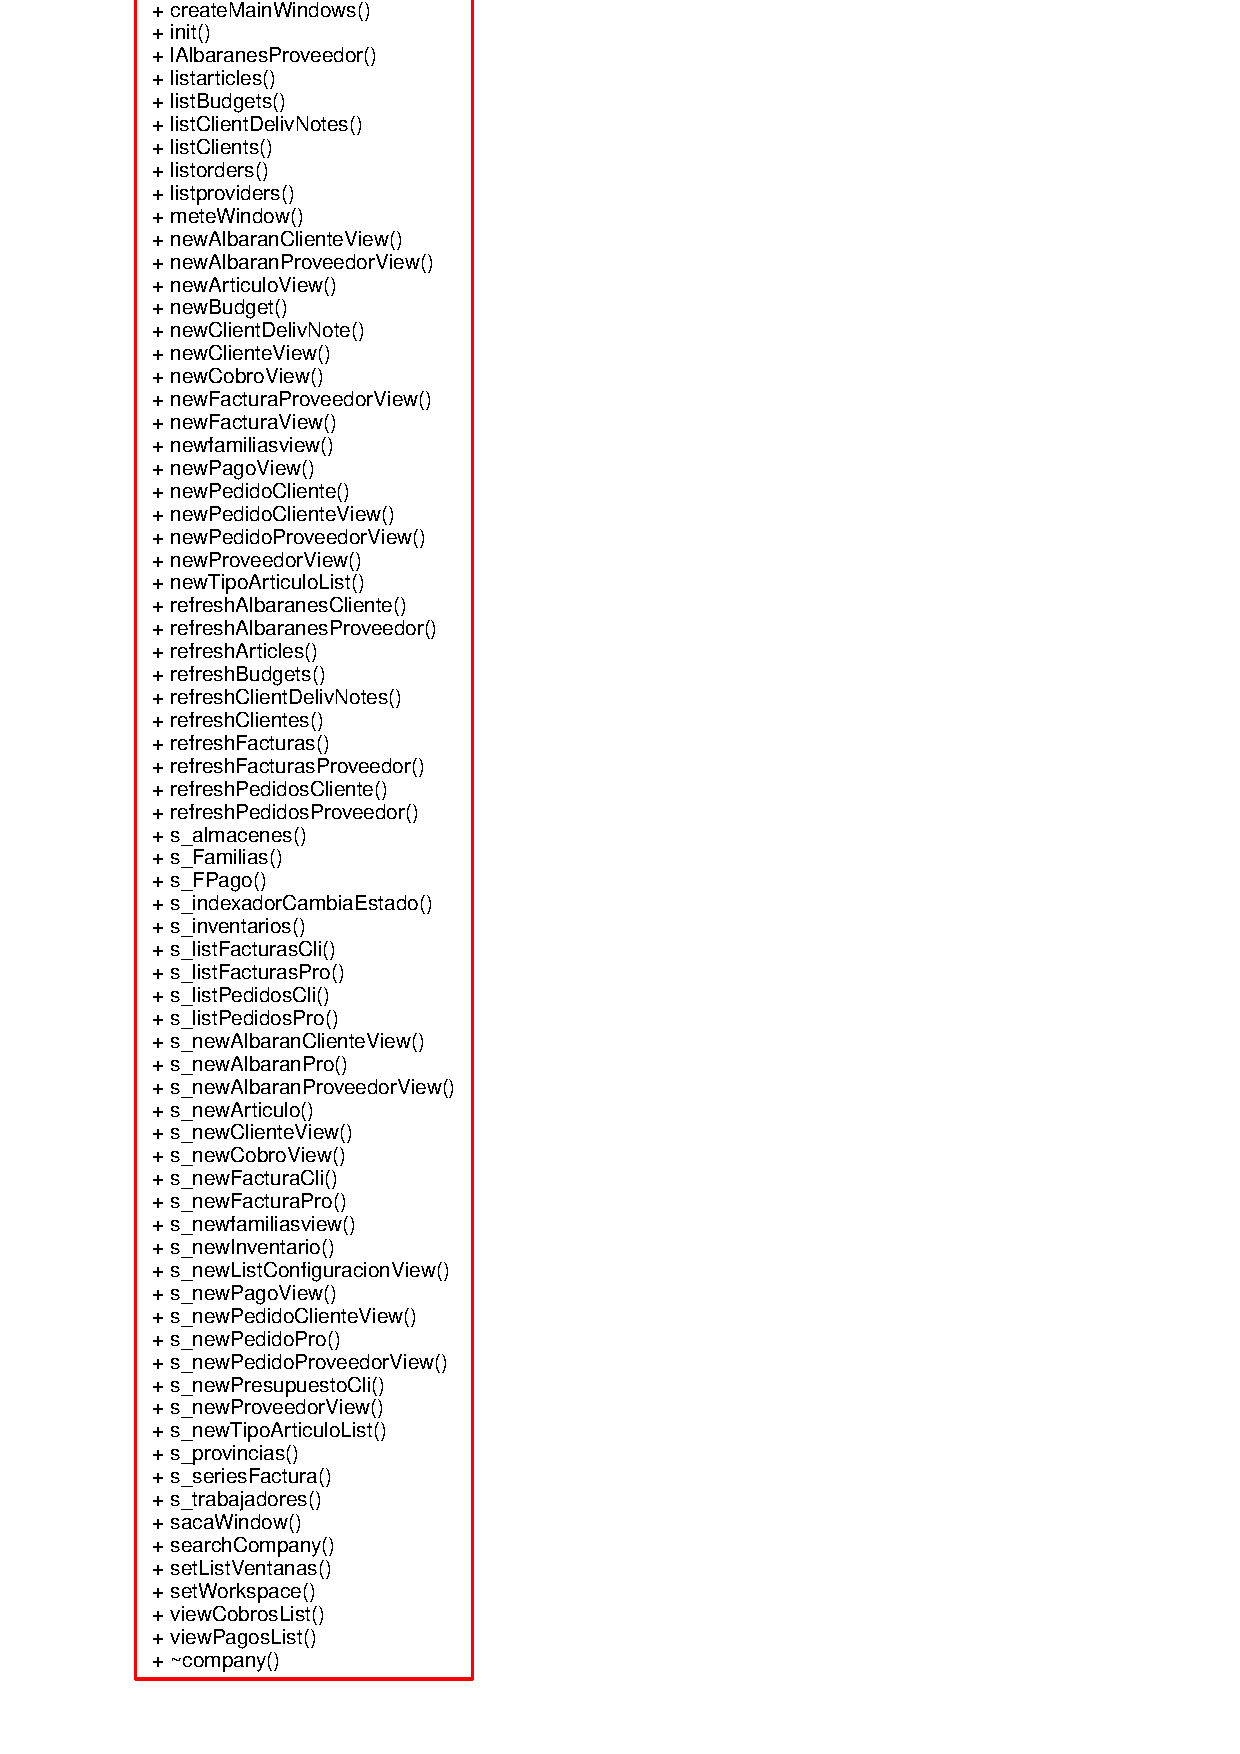
\includegraphics[width=131pt]{classPagosList__coll__graph}
\end{center}
\end{figure}
\subsection*{Slots p\'{u}blicos}
\begin{CompactItemize}
\item 
virtual void {\bf on\_\-mui\_\-actualizar\_\-clicked} ()\label{classPagosList_i0}

\item 
virtual void {\bf on\_\-mui\_\-borrar\_\-clicked} ()\label{classPagosList_i1}

\item 
virtual void {\bf on\_\-mui\_\-configurar\_\-toggled} (bool checked)\label{classPagosList_i2}

\item 
virtual void {\bf on\_\-mui\_\-crear\_\-clicked} ()\label{classPagosList_i3}

\item 
virtual void {\bf on\_\-mui\_\-editar\_\-clicked} ()\label{classPagosList_i4}

\item 
virtual void {\bf on\_\-mui\_\-imprimir\_\-clicked} ()\label{classPagosList_i5}

\item 
virtual void {\bf on\_\-mui\_\-list\_\-cell\-Double\-Clicked} (int, int)\label{classPagosList_i6}

\item 
virtual void {\bf on\_\-mui\_\-list\_\-custom\-Context\-Menu\-Requested} (const QPoint \&)\label{classPagosList_i7}

\end{CompactItemize}
\subsection*{M\'{e}todos p\'{u}blicos}
\begin{CompactItemize}
\item 
QString {\bf genera\-Filtro} ()\label{classPagosList_a0}

\item 
void {\bf hide\-Botonera} ()\label{classPagosList_a1}

\item 
void {\bf hide\-Busqueda} ()\label{classPagosList_a2}

\item 
QString {\bf idpago} ()\label{classPagosList_a3}

\item 
void {\bf imprimir} ()\label{classPagosList_a4}

\item 
void {\bf mete\-Window} (QString nom, QObject $\ast$obj)\label{classPagosList_a5}

\item 
void {\bf modoedicion} ()\label{classPagosList_a6}

\item 
void {\bf modoseleccion} ()\label{classPagosList_a7}

\item 
{\bf Pagos\-List} ({\bf company} $\ast$comp=NULL, QWidget $\ast$parent=0, Qt::WFlags flag=0)\label{classPagosList_a8}

\item 
{\bf Pagos\-List} (QWidget $\ast$parent=0, Qt::WFlags flag=0)\label{classPagosList_a9}

\item 
void {\bf presentar} ()
\item 
void {\bf setcompany} ({\bf company} $\ast$comp)\label{classPagosList_a11}

\item 
void {\bf setidproveedor} (QString val)\label{classPagosList_a12}

\item 
void {\bf show\-Botonera} ()\label{classPagosList_a13}

\item 
void {\bf show\-Busqueda} ()\label{classPagosList_a14}

\end{CompactItemize}


\subsection{Descripci\'{o}n detallada}
Muestra y administra el listado de pagos. 



\subsection{Documentaci\'{o}n de las funciones miembro}
\index{PagosList@{Pagos\-List}!presentar@{presentar}}
\index{presentar@{presentar}!PagosList@{Pagos\-List}}
\subsubsection{\setlength{\rightskip}{0pt plus 5cm}void Pagos\-List::presentar ()}\label{classPagosList_a10}


Hacemos el calculo del total. 

La documentaci\'{o}n para esta clase fu\'{e} generada a partir de los siguientes archivos:\begin{CompactItemize}
\item 
pagoslist.h\item 
pagoslist.cpp\end{CompactItemize}
